\documentclass[12pt,a4paper]{article}

\usepackage{setspace}
\onehalfspacing
\usepackage{caption}
\usepackage{subcaption}
\usepackage{float}
\captionsetup[table]{font={stretch=1.5}}     %% change 1.5 as you like
\captionsetup[figure]{font=onehalfspacing}    %% change onehalfspacing as you like
\usepackage[english]{babel}
\usepackage[utf8]{inputenc}
\usepackage{amsmath}
\usepackage{amssymb}
\usepackage{graphicx}
\usepackage[colorinlistoftodos]{todonotes}
\usepackage[top=0.75in,left=0.75in,right=0.75in,bottom=0.75in]{geometry}
\usepackage{multicol,caption}
\usepackage{makeidx}
\usepackage{pdfpages}
\usepackage[compat=1.0.0]{tikz-feynman}
\usepackage{hyperref}
%\usepackage{LuaLaTeX}
\makeindex
%\usepackage{fixltx2e}
\usepackage{cite}
\newenvironment{Figure}
  {\par\medskip\noindent\minipage{\linewidth}}
  {\endminipage\par\medskip}
\setlength{\columnsep}{1cm}
\setlength{\parindent}{0pt}
\usepackage{color,soul}
\usepackage{booktabs}
\newcommand{\ra}[1]{\renewcommand{\arraystretch}{#1}}

\title{Overview and Literature survey}
\date{\today}
\author{Ronald Collins ID:200948843}

\begin{document}
\maketitle

\begin{Figure}
 \centering
 
\includegraphics[width=1.0\linewidth]{Liverpool_logo}
 \captionof*{figure}{} 
\end{Figure}


\begin{center}
\textit{Department of Physics, High Energy Physics\\}
\textit{VIDARR collaboration\\}
\end{center}


\pagenumbering{gobble}
\newpage
\pagenumbering{roman}
\begin{abstract}
\normalsize A basic overview\\

\providecommand{\keywords}[1]{\textbf{\textit{Keywords:}} #1} %Keywords command has to be supplied manually
\keywords{Monte Carlo, Geant4, High performance computing (HPC), Anti-neutrino}
\end{abstract}
\vspace{5mm} %5mm vertical space before main body of text
%\begin{multicols}{2}
\tableofcontents
\newpage

\pagenumbering{arabic}

\section{Discovery of neutrinos}
\subsection{Theoretical Development}
%history of neutrino: \cite{griffiths2008introduction} \cite{lederman1970resource}
%\\beta decay of tritium (book cannot find, may have to replicate): \cite{lewis1970neutrinos} especially as Fermi mentions it in \cite{Fermi:1934hr}, \cite{wilson1968fermi} 
%\\Neutron proposed by Chadwick in 1932 describing a proton like recoil and odd behaviour of neutrons that can only be described by a neutron or the breaking of conservation of momentum and energy!: \cite{chadwick1932possible}. Important for giving full context to the neutrino discovery
%\\Fermis paper proposing this beta decay after Chadwick's discovery of the neutron is given in \cite{Fermi:1934hr} which proposes a neutrino and is published through Springer and the English translation from 1968 is given in \cite{wilson1968fermi}
%\\So far very little from Pauli need to include him somewhere the neutrino was his idea \cite{lederman1970resource} may have something...
The neutrino was proposed as by Pauli in 1931 as a way to conserve the energy of $\beta$ decay and to conserve the angular momentum of the products of $\beta$ decay \cite{griffiths2008introduction}\cite{lederman1970resource}. At the time beta decay was described by equation \ref{oldBetaDecay}. Where A and B represent the decaying particles, as the neutron had not yet been discovered by this point, it was considered a reaction between two nuclei. The conservation of energy dictates that the kinetic energy of the electron should only have a single value as shown in equation \ref{constant_ke_e_equation}. However, when the kinetic energy of the electron was measured \ref{beta_spectrum} the energy of the electron was not constant as seen in figure \ref{beta_spectrum} \cite{griffiths2008introduction} \cite{lewis1970neutrinos}. Equation \ref{constant_ke_e_equation} represents the maximum possible energy available to the electron in figure \ref{beta_spectrum} suggesting a third body in $\beta$ decay \cite{griffiths2008introduction}.


\begin{equation}
    A \rightarrow B + e^-
    \label{oldBetaDecay}
\end{equation}

\begin{equation}
    E = \left( \frac{{m_A}^2 - {m_B}^2 + {m_e}^2}{2m_A}\right) c^2
    \label{constant_ke_e_equation}
\end{equation}

\begin{figure}[H]
 \centering
 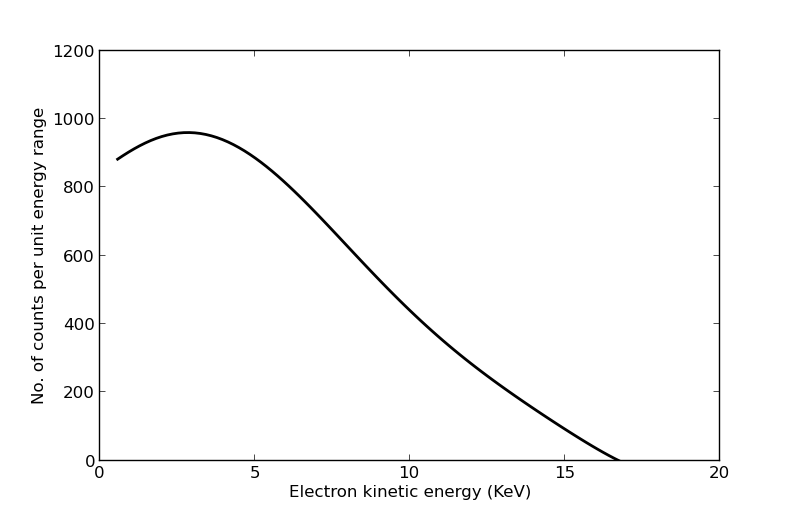
\includegraphics[height=90mm]{beta_spectrum.png}
 \captionof{figure}{$\beta$ spectrum from \cite{griffiths2008introduction} originally from \cite{lewis1970neutrinos}. The energy of the $e^-$ from $\beta$ decay varies significantly suggesting a 3 body decay model for $\beta$ decay instead of a 2 body model.} %~can be used as a kind of place holder in latex
 \label{beta_spectrum}
\end{figure}

The beta spectrum shown in figure \ref{beta_spectrum} was the first indirect evidence that neutrinos may exist. However Pauli waited until Chadwick's discovery of the neutron in 1932 \cite{chadwick1932possible} before publishing in 1934 \cite{lederman1970resource}. The complete picture of a proton-neutron nucleus allowed Enrico Fermi to produce a comprehensive theory of $\beta$ decay which incorporated Pauli's neutrino into $\beta$ decay \cite{lederman1970resource} \cite{Fermi:1934hr}. Note: a translation of Fermi's work was used \cite{wilson1968fermi}. This more complete picture made sure to differentiate the particles of the nucleus (protons and neutrons) with particles that were not bound to it (electrons and neutrinos) \cite{Fermi:1934hr} \cite{wilson1968fermi}. This period however leaves us with a mass-less neutrino which has spin 1/2 \cite{lederman1970resource}. The discovery of neutrino oscillations which will be mentioned later in section \ref{section_neutrino_oscillations} indicate that neutrinos do have mass but they were discovered far after this \cite{griffiths2008introduction}. The equation of $\beta$ decay was now given by equation \ref{semi_modern_beta_decay}. The discovery of lepton number and anti-netrinos had not yet been made however and so that quantity is not conserved in equation \ref{semi_modern_beta_decay}. 

\begin{equation}
    n \rightarrow p^+ + e^- + \nu
    \label{semi_modern_beta_decay}
\end{equation}

\subsection{Direct Measurements}
%propossal of cowan and riens using a large liquid scintillator detector: \cite{reines1953proposed}
%\\First detection: \cite{reines1953detection}
%\\distingiusing the neutrino and anti-neutrino \cite{davis1959attempt}
%\\Need to find cloud chamber pictures showing the conservation of momentum \cite{griffiths2008introduction} shows them, need to find direct source. \cite{griffiths2008introduction} also goes on to explain why this matters.
%\\ \cite{michel1949energy} supposedly does show this, but I'm having trouble getting my hands on it, UoL doesn't have access to nature papers! So will just have to include a picture from \cite{griffiths2008introduction} and clarifiy it is from \cite{michel1949energy}.
%\\ There is also the suggestion from cowan early on that anti-neutrinos and neutrinos are differing particles,  \cite{cowan1957test}, however this is by no means certain it is possible that neutrinos and anti-neutrinos are differing spin states of the same particle.
%\\ There is also the early suggestion of neutrinos and anti neutrinos being separated by a certain quantity suggested by \cite{konopinski1953universal} under a universal interaction. They use muons to suggest that certain reactions are not possible, this would later come to be known as lepton number. \\\\
%Suggestions of differing types of neutrino supposedly come from the Soviet union in 1960 but this has been lost to the iron curtain unfortunately I could not find the paper myself. The earliest reference I found is \cite{pontecorvo1963neutrino} in 1963 talking about how this influences astrophysics. 
%\\The direct measurement of differing types of neutrinos was done by \cite{DanbyG1962PhysRevLett.9.36} in 1962. This was done with a pion beam striking a beryllium target and a 10 ton spark chamber behind the target in order to pick up 37 events of one reaction and not another. They also make reference to kions but seem less certain about those due to experimental limitations. They call this the ``The neutrino flip hypothesis.'' This is a really important paper.\\

Experimental evidence for a neutrino had been observed as early as 1949, in figure \ref{pion_path} it is possible to see the impact of the neutrino. The neutrino itself is neutral and so does not show in the emulsion in figure \ref{pion_path} however the effect of the neutrino can be seen both in how the pion decays into a muon and how the muon decays into an electron \cite{griffiths2008introduction}. Collisions in the emulsion cannot account for the 90$^o$ change in direction as the particles decay, collisions can only account for dithering not abrupt changes in direction \cite{griffiths2008introduction}. At the time it was piratical to assume that the pion decay shown in equation \ref{pion_nolepNo_decay} and the muon decay shown in equation \ref{muon_nolepNo_decay} both produced the same particle when decaying. The neutrino $\nu$ \cite{griffiths2008introduction}. However as seen in equations \ref{pion_nolepNo_decay} and \ref{muon_nolepNo_decay} lepton number and neutrino flavour were not yet known and so were not conserved.
\begin{equation}
    \pi \rightarrow \mu + \nu
    \label{pion_nolepNo_decay}
\end{equation}
\begin{equation}
    \mu \rightarrow e^- + 2\nu
    \label{muon_nolepNo_decay}
\end{equation}
\\
\begin{figure}
 \centering
 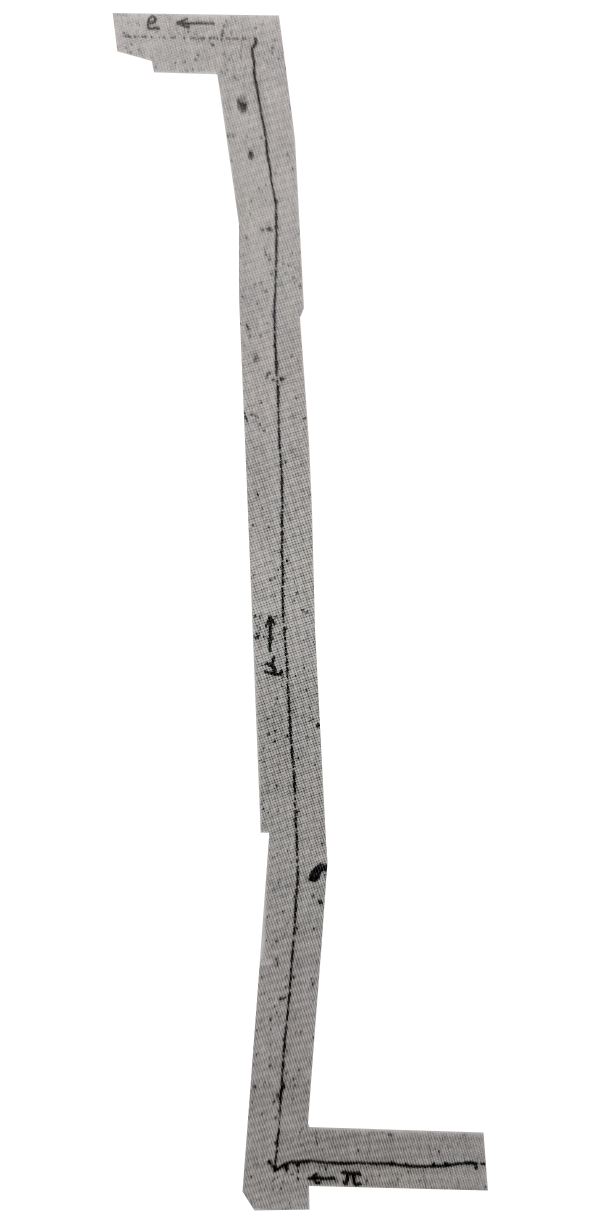
\includegraphics[height=90mm]{less_detailed_proper_path.png}
 \captionof{figure}{Path of pion decaying to a muon emitting one anti-neutrino (equation \ref{pion_nolepNo_decay}) and then that muon decaying into an electron emitting a neutrino and an anti-neutrino (equation \ref{muon_nolepNo_decay}). The paths at 90$^o$ show particle decay, collisions cannot account for this. From \cite{griffiths2008introduction} originally from \cite{michel1949energy}.} %~can be used as a kind of place holder in latex
 \label{pion_path}
\end{figure}
The first direct detection of a neutrino would be 22 years after it's initial proposal in 1931. In 1953 Cowan and Reines proposed a neutrino detector that used large amount of liquid scintillator to detect neutrinos \cite{reines1953proposed}. This proposal was followed up the same year with a cadmium loaded scintillation detector that used a delayed coincidence measurement allowing for the reduction of background \cite{reines1953proposed} \cite{reines1953detection}. The detector worked by looking for inverse $\beta$ decay shown in equation \ref{no_lepNo_dirac_inverse_beta_decay}, though the different flavours of neutrinos were not yet known. The source of the neutrinos was a reactor at Hanford \cite{reines1953detection}. This resulted in a difference counting rates in the delayed time channels of 0.41 $\pm$ 0.20 counts/min due to the pile \cite{reines1953detection}. This result was later confirmed in 1956 at the Savanaah River Plant \cite{Cowan1956Confirmation}. This new detector used a combination of liquid scintillator in three layers and cadmium chloride doped water in another two layers in a ``club-sandwich'' arrangement. This resulted in an unambiguous measurement of 0.56 $\pm$ 0.06 counts per hour with a signal 20 times higher than the accidental background associated with the reactor \cite{Cowan1956Confirmation}. 
\begin{equation}
    \Bar{\nu} + p^+ \rightarrow n + e^+
    \label{no_lepNo_dirac_inverse_beta_decay}
\end{equation}
However, the difference between neutrinos and anti-neutrinos was not yet clearly known. There are two possible hypotheses: Majorana neutrinos where the neutrino and the anti-neutrino are the same particle and Dirac neutrinos where they are distinct particles \cite{griffiths2008introduction} \cite{cowan1957test}. The possibility of Majorana neutrinos was questioned as measurements of double $\beta$ decay were found to conflict with the hypothesis \cite{cowan1957test}. Suggesting that the lifetime of such a particle would be too short compared to measurements made \cite{cowan1957test}. A direct attempt at measuring the difference between neutrinos and anti-neutrinos was made in 1959 \cite{davis1959attempt}. The experiment relied on using $Cl^{37}$ and then measuring the amount of $Ar^{37}$ produced. From previous experiments \cite{Cowan1956Confirmation} equation \ref{no_lepNo_dirac_nu_capture} was known to occur but it was not known if equation \ref{no_lepNo_maj_nu_capture} occurred. If equation \ref{no_lepNo_maj_nu_capture} was not observed then Majorana hypothesis was unlikely as $\nu$ and $\Bar{\nu}$ were probably distinct particles \cite{griffiths2008introduction} \cite{davis1959attempt}. Candidates for equation \ref{no_lepNo_maj_nu_capture} were observed 20 times below what would be expected for the Majorana hypothesis \cite{davis1959attempt}. Therefore, Dirac neutrinos were considered to be the more accurate model. 
\begin{equation}
    n + \nu \rightarrow p^+ + e^-
    \label{no_lepNo_dirac_nu_capture}
\end{equation}
\begin{equation}
    n + \Bar{\nu} \rightarrow p^+ + e^-
    \label{no_lepNo_maj_nu_capture}
\end{equation}
\\This experimental result had been predicted years prior by \cite{konopinski1953universal} which proposed a ``universal interaction'' for ``light'' and ``heavy'' particles. An undetermined phase factor c was represented as $c_P=c_N=c_H$ and $c_e=c_\mu=c_\nu=c_L$ where L and H stand ``light'' and ``heavy'' respectively. In addition to this the muon decays were suggested to give out two differing types of neutrinos shown in equation \ref{noLep_dirac_mu_decay} \cite{griffiths2008introduction}, \cite{konopinski1953universal}. Both of these observations would later be consolidated into a quantity known as lepton number with $L=+1$ for $e^-$, $\mu^-$ and $\nu$ $L=-1$ for $e^+$, $\mu^+$ and $\Bar{\nu}$ \cite{griffiths2008introduction}. 
\begin{equation}
    \mu^- \rightarrow e^- + \nu + \Bar{\nu}
    \label{noLep_dirac_mu_decay}
\end{equation}
\\However the conservation of flavours was not yet known as seen in equation \ref{noLep_dirac_mu_decay} \cite{griffiths2008introduction}. There were hints that a flavour conservation was necessary as equation \ref{mu_forbiden_decay} was never observed. When a muon decays into an electron two neutrinos must be emitted as seen in equation \ref{noLep_dirac_mu_decay}. The sharp 90$^o$ changes in direction with no other particles visible in the emulsion seen in figure \ref{pion_path} are the only observed mechanism for muon decay into an electron. This lead to the suggestion that the neutrinos emitted by the decay of muons into electrons were of different types $\nu \not= \nu'$ \cite{Lee:1960tja} \cite{griffiths2008introduction}. This would lead to a redefining of the lepton numbers to include flavours such that: $e^- L_e = +1$, $e^+ L_e = -1$, $\mu^- L_\mu = +1 $, $\mu^+ L_\mu = -1 $. With this understanding equation \ref{noLep_dirac_mu_decay} became equation \ref{proper_mu_decay}.
\begin{equation}
    \mu^- \not\to e^- + \gamma
    \label{mu_forbiden_decay}
\end{equation}
\begin{equation}
    \mu^- \rightarrow e^- + \nu_\mu + \Bar{\nu}_e
    \label{proper_mu_decay}
\end{equation}
\\An experiment to measure the differing types of neutrinos was then performed in 1962 \cite{DanbyG1962PhysRevLett.9.36}. This experiment used a pion beam striking a beryllium target and using 10 one ton spark chambers to measure the results. If $\nu_e = \nu_\mu$ then reactions \ref{test_e_decay} and \ref{test_mu_decay} should occur at equal rates \cite{DanbyG1962PhysRevLett.9.36}. The neutrino ``beam'' used produced 34 muons in the spark chamber 5 of which were considered to be background due to cosmic rays. Therefore $\sim$ 29 $e^-$ events were expected to be produced if $\nu_e = \nu_\mu$ however only 6 candidates were identified \cite{DanbyG1962PhysRevLett.9.36}. To further prove that $\nu_e \not= \nu_\mu$ two of the one ton spark chambers were tested at the Cosmotron, which did produce $e^-$s similar to what would have been expected if $\nu_e = \nu_\mu$. The results showed that these events looked very different from the 6 candidate reactions observed from the pion beam \cite{DanbyG1962PhysRevLett.9.36}. The conclusion that $\nu_e \not= \nu_\mu$ was the most likely conclusion, meaning that there were at least two different flavours of neutrinos \cite{DanbyG1962PhysRevLett.9.36}. 
\begin{equation}
    \begin{split}
    \nu + n \rightarrow p + e^- \\
    \Bar{\nu} + p \rightarrow n + e^+
    \label{test_e_decay}
    \end{split}
\end{equation}
\begin{equation}
    \begin{split}
    \nu + n \rightarrow p + \mu^-  \\
    \Bar{\nu} + p \rightarrow n + \mu^+
    \label{test_mu_decay}
    \end{split}
\end{equation}

\section{Neutrino Flavours}
\subsection{Solar Neutrinos}
\subsection{Neutrino oscillations} \label{section_neutrino_oscillations}
\subsection{Mixing Angles}

\section{Anti-neutrino Reactor Monitoring}
\subsection{Anti-neutrino Production}
\subsection{Anti-neutrino Detection}

\section{Existing Reactor monitoring programs}
\subsection{Double Chooz}
\subsection{Watchman}
\subsection{Nucifier}
\subsection{SOLID}
\subsection{Chandler}
\subsection{PANDAS}
\subsection{VIDARR}

\bibliography{refs} 
\bibliographystyle{ieeetr}

\end{document}
